% Chapter Template

\chapter{Results and Discussion} % Main chapter title

\label{Chapter6} % Change X to a consecutive number; for referencing this chapter elsewhere, use \ref{ChapterX}

\lhead{Chapter 6. \emph{Results and Discussion}} % Change X to a consecutive number; this is for the header on each page - perhaps a shortened title

%----------------------------------------------------------------------------------------
%	SECTION 1
%----------------------------------------------------------------------------------------
So far, we have developed an advanced probabilistic model that is able to infer user's behavior from smartphone logs. We exposed in details its nice properties and the theoretical advantages it has with respect to the other probabilistics models. To evaluate its performance in completing this task, we decide to confront it to state of the art current methods for doing the same job. To have a rigorous overview, we considered different methods relying on different approaches. In particular, we considered an advanced new approach of matrix factorization that was used by recent researches ($LCBMF$) and that was shown to perform well. Moreover, we considered the state of the art probabilistic approach in hidden class modeling ($LDA$) that showed impressive results since years in representing latent clusters from an observable data.

\noindent
We also discussed in details meaningfull metrics that can be used to objectively compare the performance of these models.

In this chapter, we introduce the dataset used to test these models. Then, we present the results obtained by the different models($DLMR$, $LMR$, $LCBMF$, $SVD$).

%----------------------------------------------------------------------------------------
%	SECTION 1
%----------------------------------------------------------------------------------------

\section{Presenting the Dataset}

We test our models on smartphone logs of five different users. Those smartphone logs belong to five Sony employees in Tokyo and were recorded using an internal Sony software.

\noindent
Those logs contain the records of the users during several months of observation (seven months for the newest user and ten months for the oldest). Each record represents one hour of the period of the observation. The table~\ref{duration} presents the duration of the observation period of the different users.

\begin{table}[H] 
\centering
\begin{tabular}{|l|c|c|c|c|c|}
  \hline
  &User 1 & User 2 & User 3 & User 4 & User 5 \\
 \hline
  Period & 300 & 231 & 229 & 249 &  224 \\
 \hline
\end{tabular}
\caption {Period of observation for each user in days.} 
\label{duration}
\end{table}

Those logs contain the following features :

\begin{enumerate}
\item $Activity$ that represents the activity the user is doing. It takes the values $in\_bicycle$, $in\_vehicle$, $on\_foot$, $tilting$ and $still$.
\item $Application Launch$ that represents the smartphone apps launched by the users.
\item $Bluetooth paired$ represents the bluetooth devices paired with the smartphone of the user.
\item $Day$ represents the day of the week of the record.
\item $Hour$ represents the time of the day of the record.
\item $Location$ represents the location of the users.
\item $Notification$ represents the notifications received by the user.
\end{enumerate}
%----------------------------------------------------------------------------------------
%	SECTION 2
%----------------------------------------------------------------------------------------

\section{Feature prediction results}
To test the different model, we divide the dataset into 80 \% for training and 20 \% for testing. We choose to make predictions on the $Location$ feature. Indeed, one can argue that many individual behaviors of a human are correlated to his location. For this reason, choosing the $Location$ feature as a target feature seems to be a natural choice. This tests the ability of the different models to guess the location in which the user is from the context described by his activity, the application launched, the notifications received, the day of the week, the time of the day and bluetooth devices paired to the smartphone. In this test target categories are $\{ $$most$ $frequent$ $location,$ $second$ $most$ $frequent$ $location$$,$ $other$$\}$. 
Note that for most users, $Home$ is the most frequent location and $Work$ the second most frequent location or the opposite.
\\For each model, we run the prediction tests for the 5 users and then we average the prediction accuracies results (accuracy and average accuracy) between the 5 users. For each user, the predicted location is a good prediction if it belongs to the right category (and bad prediction otherwise).

Figures ~\ref{acc} and ~\ref{avacc} shows, respectively, the accuracy and average accuracy prediction results of the five models ($DLMR$, $LMR$, $LDA$, $LCBMF$ and $SVD$) tested for different number of behaviors (i.e hidden classes).

\begin{figure} [!ht]
\centering
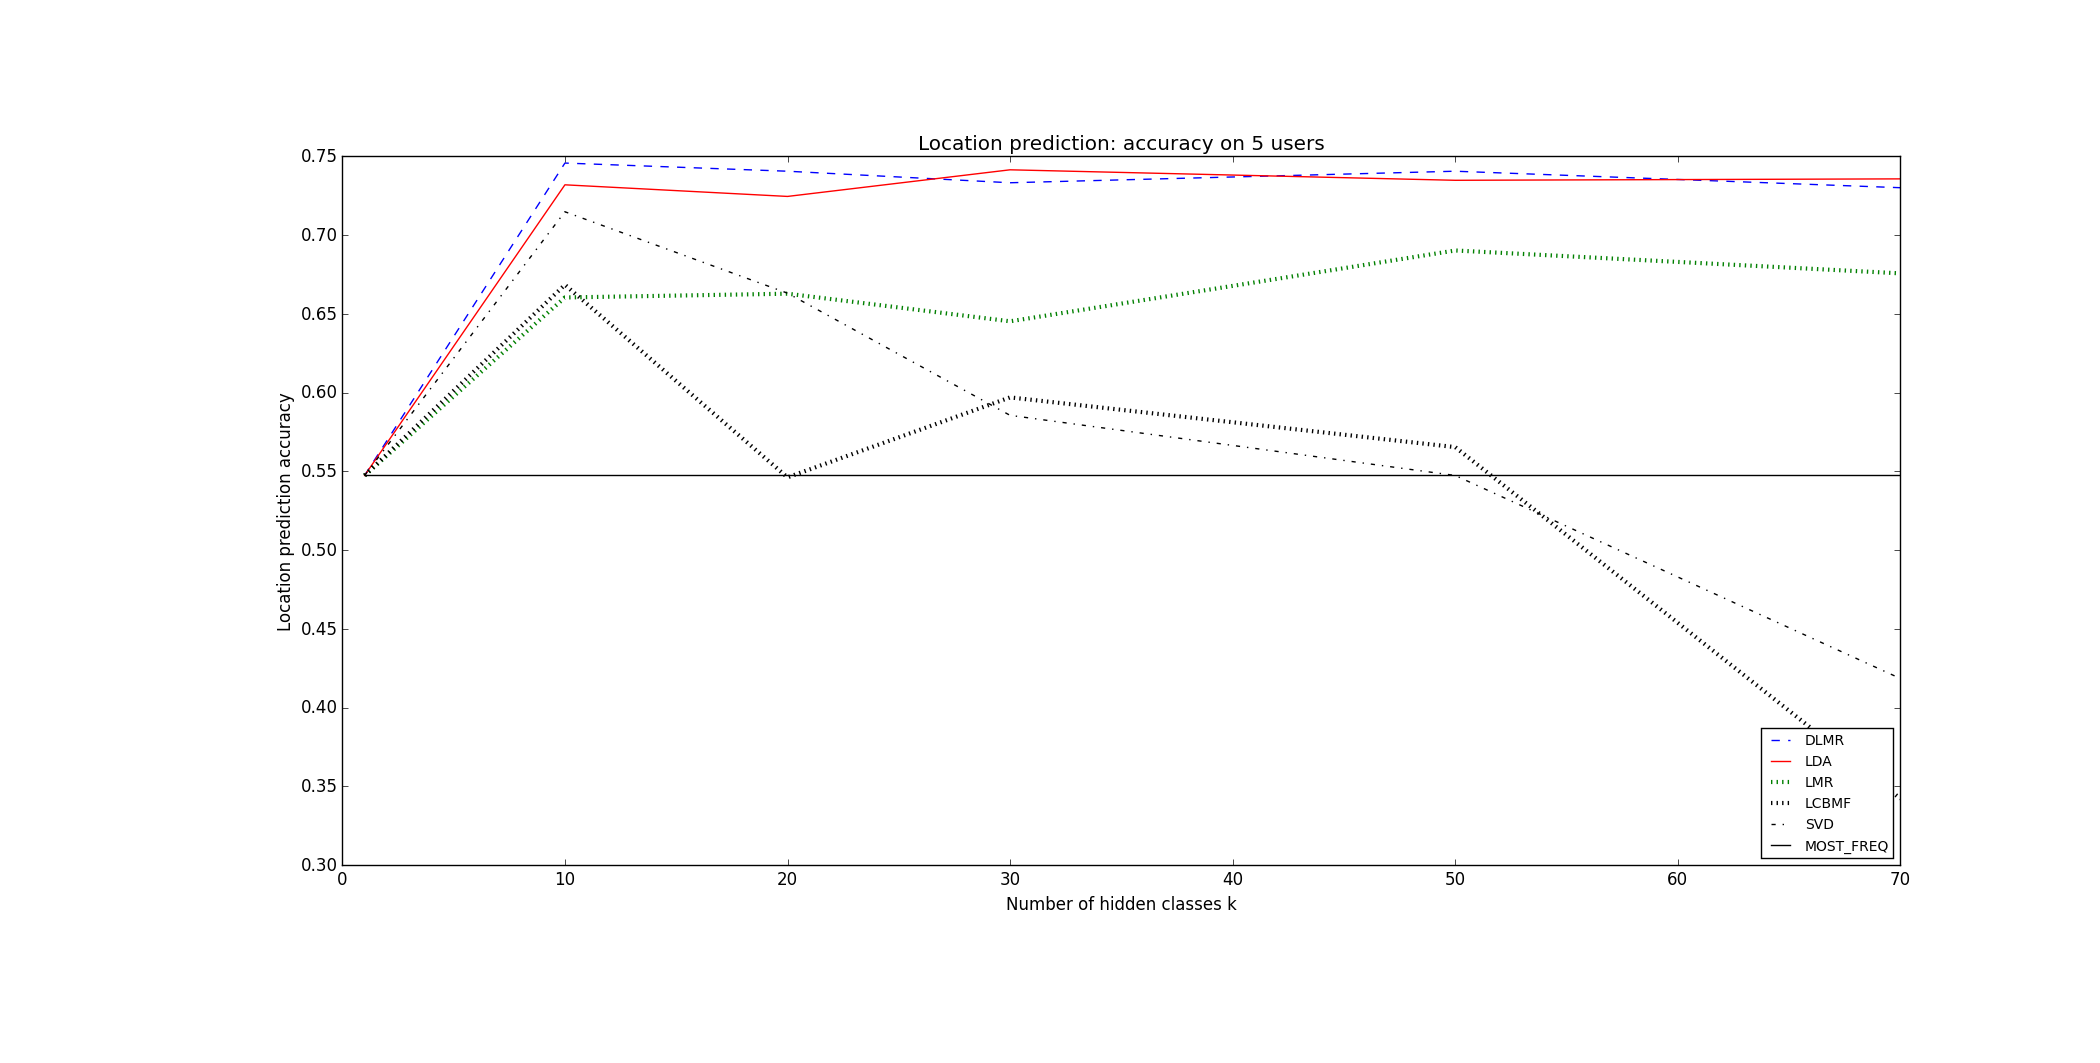
\includegraphics[scale=0.3]{Figures/location_accuracy.png}
\caption{Accuracy results of the prediction of the five models.}
\label{acc}
\end{figure}

\begin{figure} [!ht]
\centering
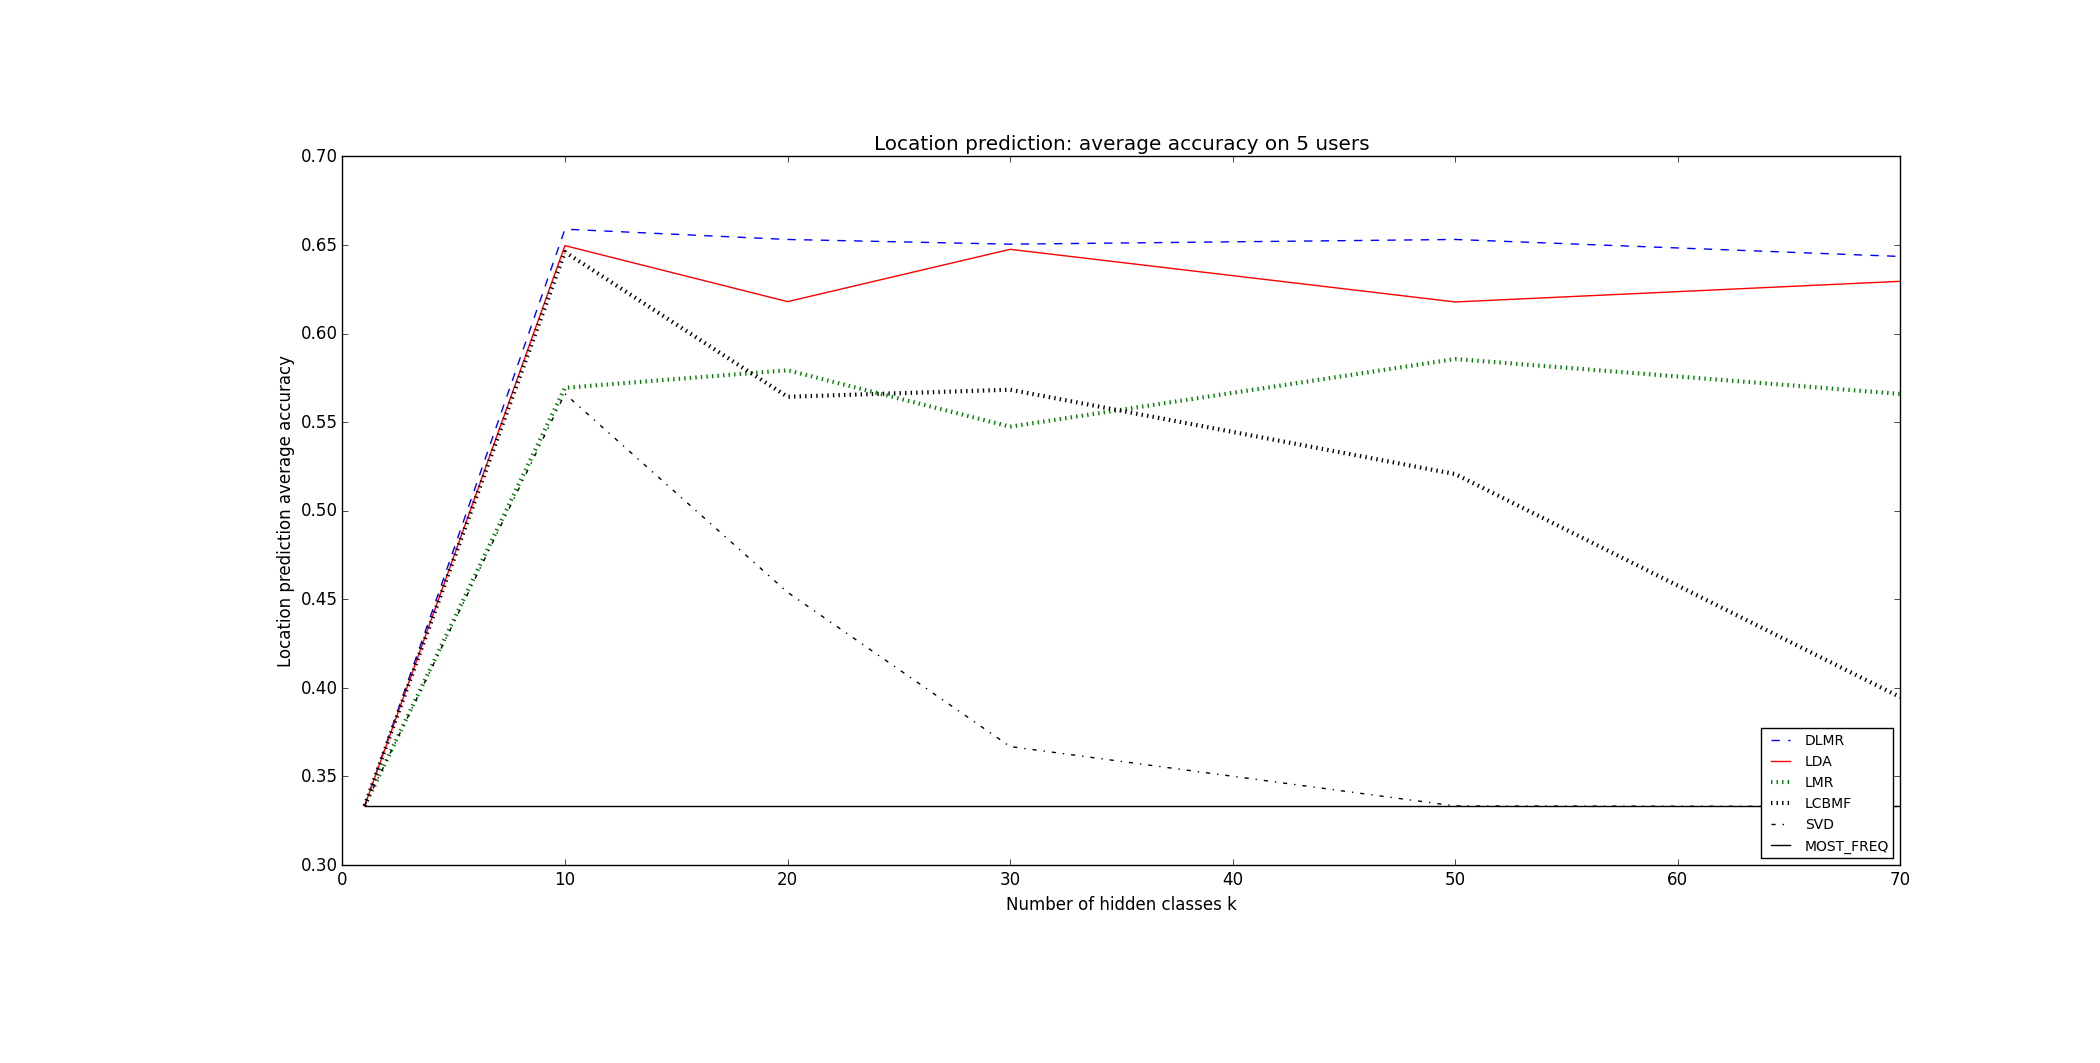
\includegraphics[scale=0.3]{Figures/location_average_accuracy.png}
\caption{Average accuracy results of the prediction of the five models.}
\label{avacc}
\end{figure}

First, we can see that the three probabilistic models, $DLMR$, $LDA$ and $LMR$ perform widely better than the matrix factorization models $LCBMF$ and $SVD$.
\\Indeed, when the number of behaviors increases ($K\geqslant 10$) the performance of $SVD$ and $LCBMF$ decreases heavily whereas $DLMR$ $LDA$ and $LMR$ stay relatively stable. This might be due to an effect of overfitting. \par

Deepen our observation int the three probabilistic models, we can see that $DLMR$ largely outperforms $LMR$. Indeed, the prediction scores of $DLMR$ are about 10\% better than $LMR$ for both average accuracy and accuracy for all the number of behaviors K. This confirms the intuition developed in chapter 3. While $LMR$ learns the behaviors expressed specifically by the records seen, $DLMR$ tries to catch a more general structure of the corpus by learning how the seen records generate the behaviors. This allows $DLMR$ to describe better an unseen data. Moreover, while both models show good stability to high number of behaviors, we can observe that for $K\geqslant 50$, $LMR$ score start to decrease while $DLMR$ is still enough stable for  $K=70$. The average accuracy plot shows this effect (average accuarcy of $LMR$ decreased by 3\% between $K = 50$ and $K = 70$ while average accuracy of $DLMR$ decreased only by 1 \% between $K = 50$ and $K = 70$, which is more due to the randomness of the test and train set rather than to overfitting). The same effect is present in the accuracies plots. 
\\As explained in chapter 3, $DLMR$ has $K+I$ ($I$ is the size of the language and equals $\sum_{f=1}^{J} I_f$) parameters to estimate while $LMR$ has $KM + KV$ parameters. Thus, when K increases the number of parameters to estimate increases much faster in $LMR$ than in $DLMR$. This is what might explain the observed effect in the sense that the big number of parameters in $LMR$ caused overfitting. \par

Concerning $LDA$, we see that it is also strong to overfitting (and stronger than $LMR$) and accurate in predictions. In fact, $LDA$ underlies the same properties than $DLMR$ (learn how records generate behaviors, small number of parameters to estimate). This is what explains its performance. However, $DLMR$ performs better than $LDA$ in prediction scores. Indeed, while they perform very close, $DLMR$ performs better than $LDA$ in average accuracy while keeping a similar score (or even slightly better score) to $LDA$ in $accuracy$. This means that $DLMR$ is able to better guess less frequent categories without loosing in general accuracy. This implies that $DLMR$ is better in detecting the rare events or contexts. This is explained by the structure of the model of $DLMR$. $DLMR$ imposes the probabilities of the values belonging to the same feature to sum to 1. This represents a much more realistic approximation of the real life than $LDA$ that spreads the probabilities over the space of all possible realizations. While frequent contexts (or events) can be outlined by an acceptable model of the real life, detecting rare contexts requires a much more precise representation.
\\Finally, evaluating $DLMR$ performance independently, we see that it performs around 74\% of good guesses and 67\% of average good guesses per class. This is a good prediction performance that shows that $DLMR$ is able to predict the future actions that the user might take. This implies that $DLMR$ was able to represent and learn the general behaviors according to which a user behaves.

As a sum up, the results show that the probabilistic models developed perform better in guessing right behaviors of users than the matrix factorization models exposed. Comparing the three probabilistic models $DLMR$, $LMR$ and $LDA$, $DLMR$ shows better results than both $LMR$ and $LDA$. This confirms the intuitions developed in chapter 3 that led us to the $DLMR$ model. Finally, the accuracies rate of $DLMR$ shows good generalization performance of unseen data, and thus proves that $DLMR$ is able to discover user behaviors from their logs.


%----------------------------------------------------------------------------------------
%	SECTION 3
%----------------------------------------------------------------------------------------

\section{Feature prediction results}
We recall that the final goal that drives our work is to discover the particular behaviors of a user from his smartphone logs. In this concluding section, we close the circle by showing examples of behaviors of the $5$ users discovered by $DLMR$. \par

First of all, and as one might expect, the $5$ users exhibit behavior that are similar. Indeed, there is at least one behavior for each user representing the fact that the user works in the week days during the day. There is also others expressing the fact that users are more often at home during the weekends, and others indicating that the users are almost always at home during the night (for all the days). An example of each of these $3$ behaviors is shown for one of the users in figure~\ref{commonBehavior} . 
\\However, one could have supposed those behaviors without analyzing smartphone logs. For this reason, they are not the most interesting habits that we aim to discover. We present them here for two reasons. First, it is a way to verify that $DLMR$ was able to discover some a-priori expected behaviors (as if we label users with some behaviors and then check that $DLMR$ is able to discover them). Second, we present them to give an intuition on how exactly the behaviors are represented in $DLMR$. \par

Now, we pay attention to examples of behaviors that are more interesting in the sense that they describe a specific user's habit. For example, the behavior in figure~\ref{readSunday} shows that $user1$ likes to do some readings on Sundays night. Indeed, $Reader$ (\href{https://play.google.com/store/apps/details?id=com.sony.drbd.reader.ext.pictorial.ja&hl=fr}{link}) is the package name of a Japanese smartphone application for purchasing and reading books. Alternatively, $user1$ would play $monster$ $strike$ (\href{https://play.google.com/store/apps/details?id=jp.co.mixi.monsterstrikeUS&hl=fr}{link}) or browse in the web using his smartphone ($Boat$ $Browser$ is the package name of a web browser (\href{https://play.google.com/store/apps/details?id=com.boatbrowser.free&hl=fr}{link})). 
\\The behavior in figure~\ref{news} shows that when the $user4$ is not at work during the day (in the week days), he would probably reads some news or watch some TV program. Indeed $SmartNews$ (\href{https://play.google.com/store/apps/details?id=jp.gocro.smartnews.android}{link}), $Socialife News$ (\href{https://play.google.com/store/apps/details?id=com.sony.nfx.app.sfrc&hl=fr}{link}) and $Gunosy$ (\href{https://play.google.com/store/apps/details?id=com.gunosy.android.world}{link}) are all news applications while $TV SideView Sony$ (\href{https://play.google.com/store/apps/details?id=com.sony.tvsideview.phone&hl=fr}{link}) is a smartphone TV app.
\\Finally, we end our example review with the behavior in figure~\ref{ing} . It shows that $user2$ is often playing ingress while being in $other$ $places$ during the weekends (in the day). In fact, $Ingress$ (l\href{https://play.google.com/store/apps/details?id=com.nianticproject.ingress&hl=fr}{link}) is an augmented reality playing location based game. In other terms, ingress is a game that transforms the real world in a game map, where players go from one place to the other trying to solve challenges. That's what explains the behavior of $user2$. \par

All these examples show that $DLMR$ is able to discover user's behaviors from his smartphone logs. In other terms, it is able to decompose a user's life (smartphone logs are a subsample of user's life) as a set of behaviors that are driving his life. Moreover, it is able to do thus by extracting both general behaviors (as sleeping at home, working in the day) and by more specific habits (reading on Sundays night, playing ingress on the week end). \par

Let's take a step back and recall the initial wish that led us to try to discover users' habbits. We wanted to enable smartphones to build a personal relationship with their owner by learning to know their habits and reacting to their specific needs. Thus we conclude this part by showing how the examples discussed above could be turned out to that end. For example, the smartphone of $user1$ could suggests to him new trendy books to read on Sundays night (even if $user1$ was not planning to read, maybe because he is bored with the books he is currently reading), or even proposes new games that he could play. Concerning $user2$, if his smartphone knows that it will be rainy next Sunday, then it could alert it's owner and suggests him to schedule his ingress session in another day if he is planning to play. Those are only few examples of possible applications and are far from being exhaustive. The work developed in this thesis does not already enable smartphones to act as described (smartphones need to be able to interpret the behaviors they extracted to do so), but allowing them to catch users' behaviors is a necessary and important step towards that direction.

\begin{figure*}[t!]
    \centering
    \begin{subfigure}[t]{0.33\textwidth}
        \centering
        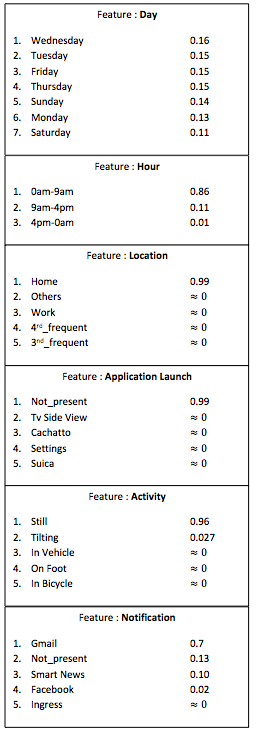
\includegraphics[scale=0.5]{Figures/Home.png}
        \caption{Home\_night.}
    \end{subfigure}%
    \begin{subfigure}[t]{0.33\textwidth}
        \centering
        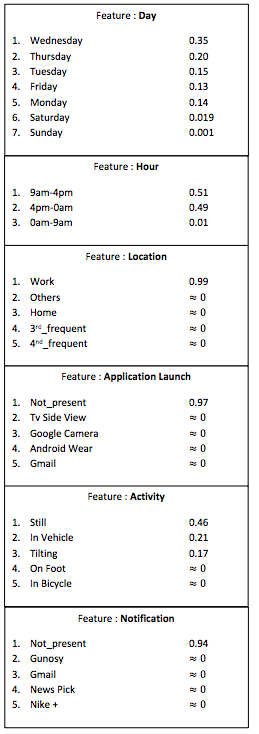
\includegraphics[scale=0.5]{Figures/Work.png}
        \caption{Working\_week\_days.}
    \end{subfigure}%
  \begin{subfigure}[t]{0.33\textwidth}
        \centering
        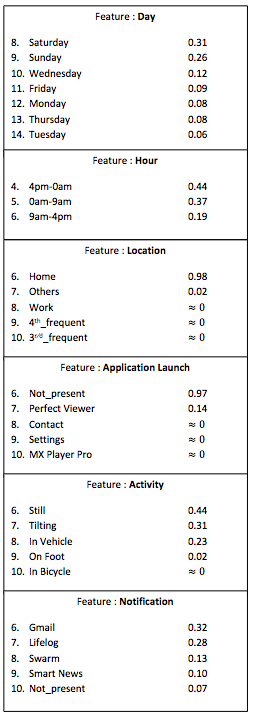
\includegraphics[scale=0.515]{Figures/Homeweekend.png}
        \caption{Home\_weekend.}
    \end{subfigure}

    \caption{Examples of common behaviors.}
\label{commonBehavior}
\end{figure*}


\begin{figure*}[t!]
    \centering
    \begin{subfigure}[t]{0.33\textwidth}
        \centering
        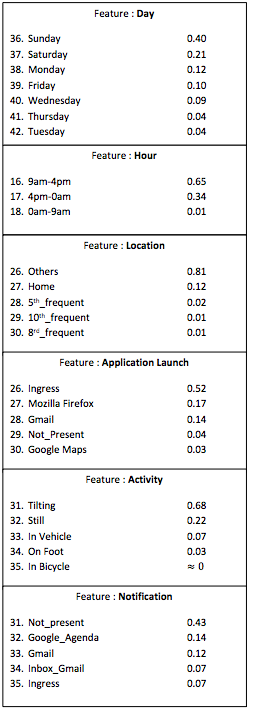
\includegraphics[scale=0.51]{Figures/Ingress.png}
        \caption{play\_ingress\_weekend.}
\label{ing}
    \end{subfigure}%
    \begin{subfigure}[t]{0.33\textwidth}
        \centering
        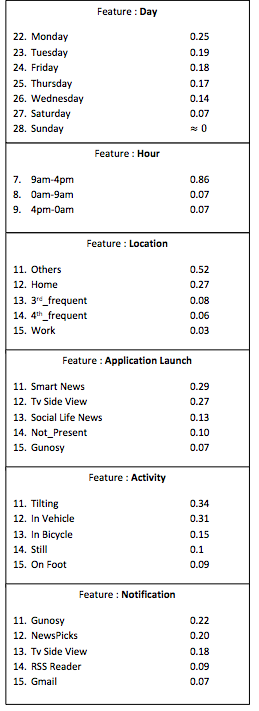
\includegraphics[scale=0.51]{Figures/News.png}
        \caption{Reading\_news\_mornings.}
\label{news}
    \end{subfigure}%
  \begin{subfigure}[t]{0.33\textwidth}
        \centering
        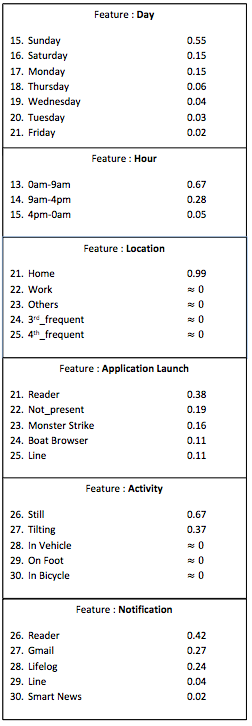
\includegraphics[scale=0.5]{Figures/sundayReading.png}
        \caption{reading\_sunday\_night.}
\label{readSunday}
    \end{subfigure}
    \caption{Examples of special behaviors.}
\label{specialBehavior}

\end{figure*}

